\subsection{Hardware Architecture and Modular Integration}
\label{sec:hardware_architecture}
The platform comprises a quadrotor, a rigid proximal mount, a single-section continuum arm, and a distal camera--gripper assembly (Fig.~\ref{fig:hardware_architecture}). The hardware arrangement distinguishes vehicle-fixed sensing and computation from the deforming arm and its rigid distal tool.

\begin{figure*}[!t]
\centering
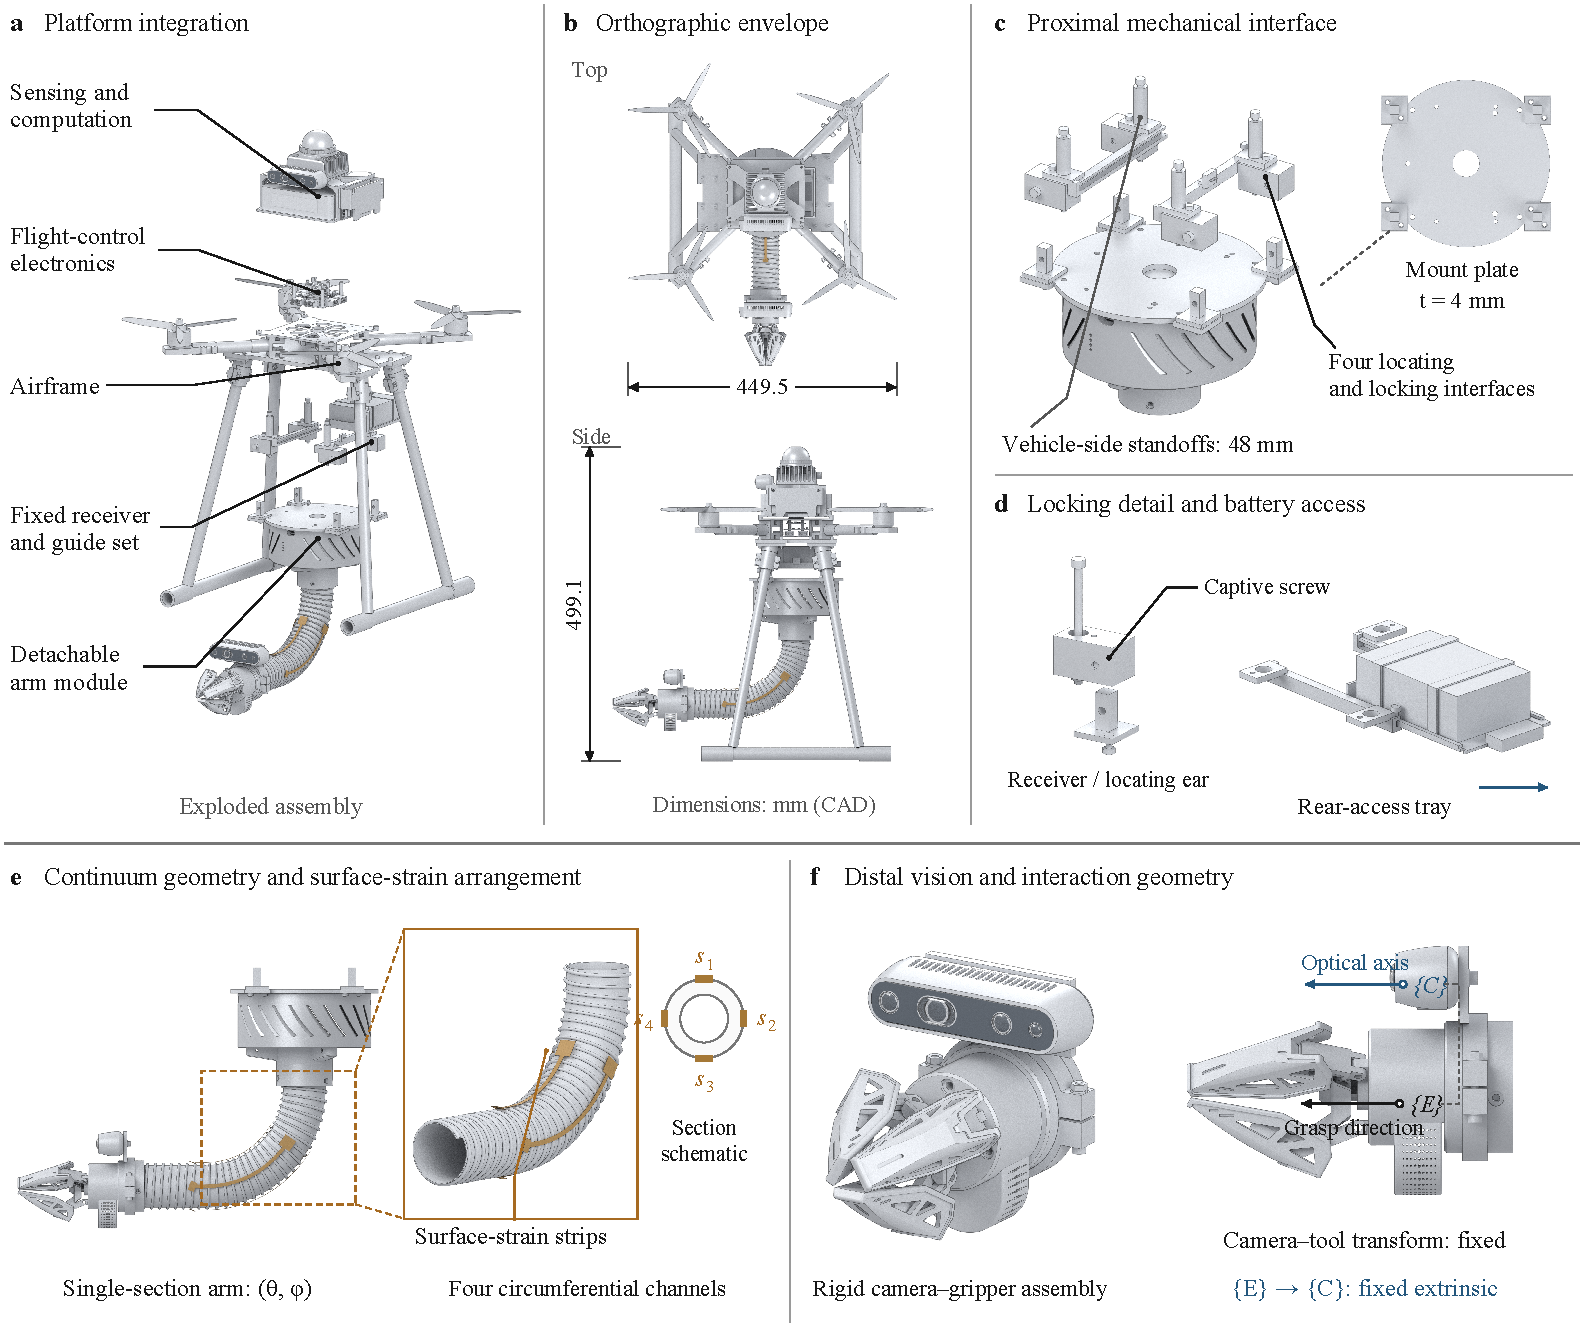
\includegraphics[width=\textwidth]{hardware_architecture_journal.pdf}
\caption{Platform integration, mechanical interfaces, and morphology sensing. (a) Native-CAD exploded assembly separating sensing/computation, flight electronics, airframe, fixed receivers, and the removable arm module. (b) Orthographic views and the envelope of the shown CAD configuration (mm). (c) Mount plate and vehicle-side standoffs. (d) Local locking interface and independent rear-access battery tray. (e) Single-section continuum module, enlarged surface-strain placement, and a schematic four-channel cross-section. (f) Distal assembly and side projection showing the fixed camera--tool relationship. All structural views use the same native CAD geometry and rendering convention. Exploded offsets illustrate assembly relationships. The LiDAR-equipped layout is the configuration for the planned map-registered flight study.}
\label{fig:hardware_architecture}
\end{figure*}

\textit{Vehicle and attachment:} The upper stack accommodates scene-facing sensors and an onboard computer, while the flight controller and power electronics occupy the central airframe. Underbody receivers engage the arm-side mounting plate through locking interfaces. The battery tray is accessed independently from the rear. Once installed, the arm mount defines a fixed vehicle-to-arm transformation; module removal is a maintenance configuration.

\textit{Morphology and distal sensing:} Four circumferential surface-strain channels observe arm deformation. The distal D435 and three-finger gripper are joined through a rigid clamp, preserving the camera-to-tool extrinsic as the continuum section bends. These observations are complementary to the body-mounted sensors: distal vision and strain support morphology estimation, while the LiDAR-equipped layout provides the scene-sensing configuration for the map-registered hardware study in Sec.~\ref{sec:hardware}.

\textit{Planning interface:} The hardware is represented by fixed mounting transforms, a morphology-dependent backbone, and the rigid distal assembly. UAV position and yaw combine with $(\theta,\phi)$ to form the six-dimensional planning state. This physical decomposition motivates the coupled occupancy model and the base-motion compensation developed below.
